\documentclass[11pt,a4paper]{article}
\usepackage[margin=25mm]{geometry}
\usepackage{amsmath,amssymb,amsthm,booktabs,microtype,hyperref,graphicx,xcolor,enumitem}
\hypersetup{colorlinks=true,linkcolor=blue!45!black,urlcolor=blue!45!black,pdftitle={UNNS-U2-TI-DYN v001},pdfauthor={UNNS Research Programme}}
\setlength{\parskip}{4pt}
\setlength{\parindent}{0pt}
\newtheorem{theorem}{Theorem}[section]
\newtheorem{proposition}[theorem]{Proposition}
\newtheorem{corollary}[theorem]{Corollary}
\newtheorem{remark}[theorem]{Remark}
\newcommand{\NN}{\mathbb N_{>0}}
\title{\textbf{UNNS-U2-TI-DYN v001}\\[4pt]\large Maximal-Neighbor Dynamics and Prime-Degree Rigidity\\in the Reversible SELECT-II Arithmetic Graph}
\author{UNNS Mathematical Foundations Research Programme}
\date{9 November 2026\\\small Independent theorem addendum to UNNS-U2-TI v001}
\begin{document}
\maketitle
\begin{abstract}
Two arithmetic statements arising during the interpretation of the frozen UNNS-U2-TI v001 target-blind experiment are proved and recorded separately. The largest neighbor of every positive integer $x$ in the reversible SELECT-II graph is $(x+1)^2$; consequently a fixed, target-blind graph-local rule produces the non-linear orbit $1,4,25,676,458329,\ldots$. Moreover, vertex degree admits an exact divisor formula and exhibits a rigidity gap: $\deg(1)=1$, primes have degree $2$, no vertex has degree $3$, and every composite has degree at least $4$. The theorems follow from the existing edge grammar without adding operators. A standalone exact-integer verifier is supplied. This addendum does not revise the frozen TI registration, claim generation of the predeclared classical sequence targets, or establish literature novelty.
\end{abstract}

\section{Context, status and scope}
The baseline UNNS-U2-TI v001 investigated a preregistered finite grammar GL-1 of target-blind graph-local selector rules. That study reported 6,720 registered orbits and no successful reproduction of the registered nontrivial target sequence families. After examining the registered outputs, an exploratory group of 448 orbits was observed to obey $x\mapsto(x+1)^2$ and was not counted as a preregistered success because of the experiment's escape threshold. The present note proves why this recurrence arises from one intrinsic graph-local ordering rule. It also documents the degree-based primality characterization, which was not a TI registration endpoint.

Evidence is distinguished throughout: \emph{proved} means the general arithmetic argument appears here; \emph{bounded computational corroboration} refers to the exact-integer verifier; \emph{exploratory} refers to the post-registered observation in TI. The frozen TI source, verifier, registration and earlier releases are not edited or repackaged in this addendum.

\section{The graph and its complete neighborhood}
\begin{proposition}[Exact neighbors]\label{prop:neighbors}
Let $G=(V,E)$, where $V=\NN$ and $E$ consists of undirected edges
\[
 \{kN,k(N+1)^2\}, \qquad k,N\in\NN.
\]
At every vertex $x$, its neighbors are exactly the disjoint union of
\begin{align}
 \mathcal F(x)&=\left\{\frac{x}{d}(d+1)^2: d\mid x\right\},\\
 \mathcal I(x)&=\left\{\frac{x}{q^2}(q-1): q\ge2,\ q^2\mid x\right\}.
\end{align}
Every element of $\mathcal F(x)$ exceeds $x$, and every element of $\mathcal I(x)$ is smaller than $x$. Both parametrizations have distinct outputs for distinct eligible parameter values.
\end{proposition}
\begin{proof}
A forward edge leaving $x$ has $x=kN$; put $d=N$. A reverse edge entering $x$ has $x=k(N+1)^2$; put $q=N+1$. These give the displayed formulas, and conversely each indicated divisibility relation gives an edge. For forward edges the ratio is
$ f(d)=(d+1)^2/d=d+2+1/d>1$. Its difference $f(d+1)-f(d)=1-1/(d(d+1))>0$ proves distinctness. For inverse edges the ratio $g(q)=(q-1)/q^2<1$ satisfies
\[
 g(q)-g(q+1)=\frac{q^2-q-1}{q^2(q+1)^2}>0\qquad(q\ge2).
\]
Thus inverse outputs are distinct. The forward and reverse sets cannot intersect, since the former are strictly larger than $x$ and the latter strictly smaller.
\end{proof}

\section{The maximal-neighbor theorem}
\begin{theorem}[Unique maximal neighbor]\label{thm:max}
For every $x\in\NN$,
\[
\boxed{\max\{y:y\sim x\}=(x+1)^2.}
\]
The maximum is unique and is attained by the forward label $N=x$.
\end{theorem}
\begin{proof}
By Proposition~\ref{prop:neighbors}, every inverse neighbor is smaller than $x$ and every forward neighbor is larger than $x$. Among eligible forward labels $d\mid x$, $f(d)$ is strictly increasing and the largest divisor is $d=x$. Thus the maximal neighbor is $x f(x)=(x+1)^2$ and is unique.
\end{proof}

\begin{corollary}[Target-blind non-linear dynamics]\label{cor:dyn}
The deterministic graph-local rule
\[
 S_{\max}(x)=\arg\max_{y\sim x}y
\]
produces, without any target input or sequence-specific table, the infinite recurrence
\[
 x_{j+1}=(x_j+1)^2. \tag{DYN}
\]
From $x_0=1$ it begins $1,4,25,676,458329,\ldots$ and is strictly increasing and nonperiodic. For $j\ge1$,
\[
 x_j\ge4^{2^{j-1}}.
\]
\end{corollary}
\begin{proof}
The recurrence follows from Theorem~\ref{thm:max}. Its next vertex is reached by the legal forward step with label $N=x_j$; evaluating this rule does not require factorization or enumerating the neighborhood. For $x\ge1$, $(x+1)^2>x$. Also $x_1\ge4$, and $x_{j+1}\ge x_j^2$ implies the stated lower bound inductively.
\end{proof}

\begin{remark}[Status relative to existing sequence literature]
The recurrence (DYN) is not a newly discovered number sequence: starting one term earlier from zero it is recorded as OEIS A004019. The result documented here is the characterization of the same recurrence as the unique maximal-neighbor selection rule for the particular reversible SELECT-II graph. No claim of priority or novelty for that graph-theoretic characterization is made without a dedicated prior-art review.
\end{remark}

\section{Exact degree and primality rigidity}
Let $\tau(x)$ be the number of positive divisors of $x$.
\begin{theorem}[Degree formula and degree gap]\label{thm:deg}
For every $x\in\NN$,
\[
\boxed{\deg_G(x)=\tau(x)+\#\{q\ge2:q^2\mid x\}.} \tag{1}
\]
If $x=\prod_p p^{e_p}$, equivalently,
\[
\boxed{\deg_G(x)=\prod_p(e_p+1)+\prod_p\left(\lfloor e_p/2\rfloor+1\right)-1.} \tag{2}
\]
In particular,
\[
\deg_G(1)=1,\qquad \deg_G(p)=2\ (p\text{ prime}),\qquad
\deg_G(x)\ge4\ (x\text{ composite}).
\]
No vertex has degree $3$. For every $x\ge2$, $x$ is prime if and only if $\deg_G(x)=2$.
\end{theorem}
\begin{proof}
Proposition~\ref{prop:neighbors} gives exactly one forward neighbor per divisor $d\mid x$ and exactly one inverse neighbor per integer $q\ge2$ with $q^2\mid x$. Distinctness and disjointness imply (1). If $x=\prod_p p^{e_p}$, then $q^2\mid x$ precisely when each $p$-exponent of $q$ is at most $\lfloor e_p/2\rfloor$. Including $q=1$ gives $\prod_p(\lfloor e_p/2\rfloor+1)$ choices, yielding (2).
For $x=1$, there is one forward neighbor. For prime $p$, there are two forward neighbors and no inverse neighbors. If $x$ is squarefree composite, it has at least two distinct prime factors, so $\tau(x)\ge4$. If $x$ is not squarefree and composite, then $\tau(x)\ge3$ and at least one nontrivial square divides $x$, making $\deg_G(x)\ge4$. These cases exhaust positive integers and establish the gap and primality equivalence.
\end{proof}

\begin{corollary}[Special arithmetic subfamilies]
If $x$ is squarefree, then $\deg_G(x)=\tau(x)$. If $x=p^e$ is a prime power, then
\[
\deg_G(p^e)=e+1+\lfloor e/2\rfloor.
\]
\end{corollary}

\begin{center}
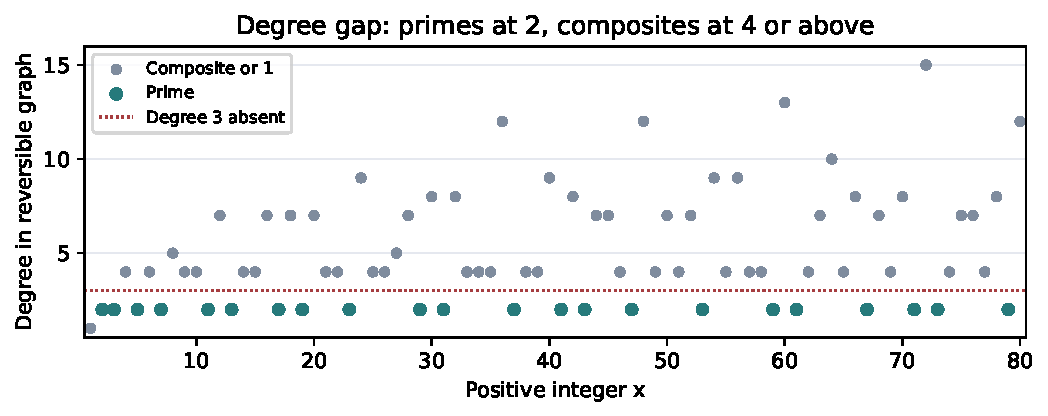
\includegraphics[width=.93\linewidth]{../figures/degree_gap.pdf}
\end{center}
\vspace{-4pt}
\begin{center}\small\textbf{Figure 1.} Exact degrees for $1\le x\le80$. Prime vertices occupy degree $2$; degree $3$ is absent.\end{center}

\section{Information locality versus computational cost}
Theorem~\ref{thm:max} has a constant-description implementation: choose $N=x$ and output $(x+1)^2$. The underlying arithmetic operations become more expensive with integer bit length, but no divisor enumeration is necessary to decide the maximal neighbor.

By contrast, Theorem~\ref{thm:deg} expresses primality as a graph-local invariant, $\deg_G(x)=2$. This is \emph{structural definability}, not a constant-time primality algorithm. Computing a complete neighborhood by the given forward/inverse labels requires identifying divisors or equivalent arithmetic information. Therefore an unrestricted ``read degree'' primitive would conceal substantial computational work unless an explicit cost model charges for obtaining that information. The TI GL-1 interpreter already enumerates neighborhoods; the theorem does not enlarge its admissible instruction set. A prime-successor selector has not been constructed or implied.

\section{Exact verifier and reproducibility}
The release includes a standalone Python-standard-library verifier (\texttt{code/verify\_dyn.py}) that (i) checks the maximal-neighbor and degree identities for all $1\le x\le10{,}000$, (ii) checks the degree gap and prime equivalence with independent trial division, (iii) compares two neighborhood enumeration implementations for all $1\le x\le1{,}200$, (iv) tests 2,500 general edge instances, and (v) replays the initial orbit. These bounded checks corroborate, but do not replace, the universal proofs above. The exact run counts and verdict are stored in \texttt{reports/verification\_report.json}.

\section{Provenance, limitations and research disposition}
This is a \emph{separate addendum} prepared after TI v001; it does not modify TI's preregistered endpoints or relabel exploratory observations as registered successes. The original TI archive hash is preserved in \texttt{PROVENANCE.json}. Two universal results are proved: (a) maximal-neighbor dynamics and (b) exact degree/primality rigidity. The orbit's recurrence has prior art, as documented above. A separate literature survey is required before claiming originality for the graph-specific formulations.

Natural follow-up questions include ranked-neighbor dynamics, structural versus algorithmic degree access, and whether any target-blind selector with explicitly charged information access generates prime or other registered target families. These remain research questions, not conclusions of this note.

\begin{thebibliography}{9}
\bibitem{TI} UNNS Mathematical Foundations Research Programme, \emph{UNNS-U2-TI v001: Target-Blind Selector Language and Generative Knowledge Accounting}, frozen project release, November 2026.
\bibitem{OEIS} The On-Line Encyclopedia of Integer Sequences, \emph{A004019}, \url{https://oeis.org/A004019} (consulted 9 November 2026).
\end{thebibliography}
\end{document}
